% status: 0
% chapter: TBD

\title{SETI$@$Home}

\author{Juliano Ferrari Gianlupi}
\affiliation{%
  \institution{Indiana University}
  \country{USA}}
\email{jferrari@iu.edu}


% The default list of authors is too long for headers}
\renewcommand{\shortauthors}{J. F. Gianlupi}


\begin{abstract}
After funding was cut SETI lauched SETI$@$Home, a public volunteer computer 
via the internet. Using this software users donate idle CPU time for SETI to do 
calculations~\cite{hid-sp18-601-www-sathome-about}. It was released in 1999 and 
one of its goals was to prove the viability of volunteer computing. This goal 
has succeded completly. SETI$@$Home was inspiration for several similar
project~\cite{hid-sp18-601-www-boinc-projects}, one of each is the 
 LHC$@$home~\cite{hid-sp18-601-www-lhc-at-home-history}.
\end{abstract}

\keywords{hid-sp18-601, setiathome}


\maketitle

\section{Introduction}\label{hid-sp18-601-section-introduction}
SETI (Search for Extra Terrestrial Intelligence) is a research institute that 
searches for signals of extra-terrestrial 
life~\cite{hid-sp18-601-paper-cocconi1959searching}. It does this mostly by 
listening to radio signals and trying to determine if they are not human made 
and neither are natural. 

As any signal coming from another sapient form of life would come from great 
distances it would be a very weak signal. In addition most of the signal picked 
up by a radio telescope that is not man made is noise, from celestial bodies 
and from the electronics of the equipment 
itself~\cite{hid-sp18-601-paper-anderson2002seti}. All of this makes finding an 
actual signal a hard endeavor, as the hypothetical alien radio message would be 
buried in that noise.

Due to the signal to noise ratio being so unfavorable SETI uses supercomputers 
to make the bulk of their calculations. In 1995 using a network of volunteer 
computers to make the calculations instead was 
proposed~\cite{hid-sp18-601-book-foster1999carl}. They use CPU time that would
be idle, meaning that users would not notice any performance difference on 
their machines. Although cheaper than a super computer this approach is 
not free. It requires a network bandwidth big enough
to handle all of the data as well as maintenance of the servers. As the 
program depends of volunteers the data sizes cannot be too large, as the users
will have to download the data~\cite{hid-sp18-601-paper-anderson2002seti}.


\section{How SETI$@$home distributes data and how the
data is analyzed}\label{hid-sp18-601-section-howworks}
\subsection{Data distribution to the network
of nodes}\label{hid-sp18-601-subsection-data-dist}
The data comes from the Arecibo radio telescope in Puerto Rico. As the facility
does not have high speed internet the data must first be send by regular mail to
 Berkeley~\cite{hid-sp18-601-www-sathome-howworks}. Once there the data is 
 divided in ``work units'', which size is 250 kibibytes, and distributed to the 
 collaborators' computers on the network.

\begin{figure*}[!htb]
        \centering
        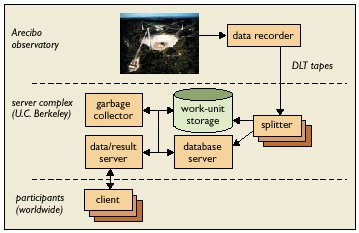
\includegraphics[width=0.35\textwidth]{figures/arecibo-to-net.jpg}
        \caption{Data preprocess and
        distribution~\cite{hid-sp18-601-paper-anderson2002seti}}\label{datasend}
\end{figure*}

The data to be analyzed are radio waves. The frequency range of the waves 
analized in the SETI$@$Home project is from 1418MHz to 1421MHz organized in 
10Khz pieces~\cite{hid-sp18-601-paper-anderson2002seti}. A work unit is 100 
seconds of the recording of one of this 
slices~\cite{hid-sp18-601-www-sathome-howworks}. How the data is to be analyzed 
will be discussed in Subsection~\ref{hid-sp18-601-subsection-nodes-work}.

Once the data is separated into work units the work units are sent to a work 
unit storage and a database server~\cite{hid-sp18-601-book-foster1999carl}. 
The database and storage communicate with a data/result server, responsible for 
communicating with the nodes, and a garbage collector, responsible for 
removing flagged data from the 
storage
~\cite{hid-sp18-601-book-foster1999carl,hid-sp18-601-paper-anderson2002seti}.

The SETI$@$home team has tried two method for selecting works units to be 
deleted. One of them is to delete units that have received \textit{N} results,
where \textit{N} is a result redundancy target. This method of deletion might 
be slower than the creation of new work units, filling up the storage and 
halting the creation of new work 
units~\cite{hid-sp18-601-paper-anderson2002seti}.

Because of this bottleneck the method has been changed to be as follows: 
If a work unit has had results received \textit{N} times and has been sent 
\textit{M} times (where $M>N$) it is selected for 
deletion~\cite{hid-sp18-601-paper-anderson2002seti}. This method has 
a downside of some work units never producing results. The fraction of work
units that don't produce results can be made small by increasing \textit{M}.

The nodes get new work units as soon as they return the results for the 
previous one. Once the results return to the main server they are recorder 
and further analyzed. Result handling has two functions, one is to 
get the scientific results~\cite{hid-sp18-601-paper-anderson2002seti}. 
Compare the results about a work unit from several nodes, to see if there 
is consensus and catch malicious results. 
If the results from different nodes are similar but not identical a 
representative result is chosen.

\begin{figure*}[!htb]
        \centering
        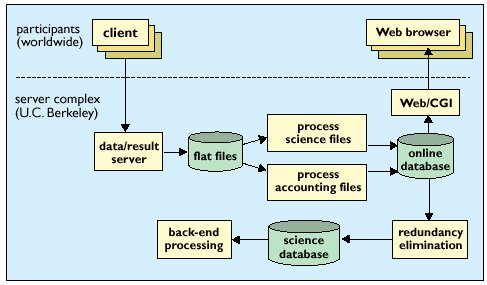
\includegraphics[width=0.35\textwidth]{figures/data-return.jpg}
        \caption{Data return and 
        postprocess~\cite{hid-sp18-601-paper-anderson2002seti}}\label{datasend}
\end{figure*}

The other function of result handling is accounting. The server creates 
log entries with information about the node, it's CPU type and user for 
instance. This is done both to flag malicious users and give credit for
the users that found an alien signal~\cite{hid-sp18-601-paper-anderson2002seti}.

\subsection{Signal type and signal distortion}\label{hid-sp18-601-subsection-signal}
\begin{figure*}[!htb]
        \centering
        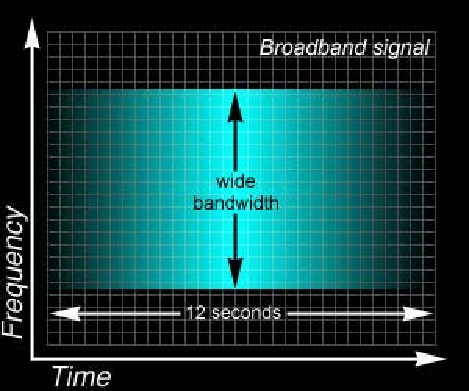
\includegraphics[width=0.35\textwidth]{figures/broadband.pdf}
        \caption{Example of a Gaussian broadband
        signal~\cite{hid-sp18-601-www-sathome-howworks}}\label{broadbandfigure}
\end{figure*}
As the degradation of a signal sent in many frequencies (broadband) is greater 
than the degradation of a narrowband 
signal~\cite{hid-sp18-601-www-sathome-interference} the SETI$@$home team looks
 for the later to be candidates for alien 
 signals~\cite{hid-sp18-601-www-sathome-howworks}. Another parameter that 
 narrows the signal search is the form it has to have in time. As the telescope 
 used by SETI$@$Home does not track the sky (meaning it is fixed) while looking 
 for extra terrestrial signals the radio wave must rise and fall in strength 
 over a period of twelve seconds, the amount of time any source object would 
 take  to pass trough the focus of the 
 telescope~\cite{hid-sp18-601-www-sathome-interference}.

\begin{figure*}[!htb]
        \centering
        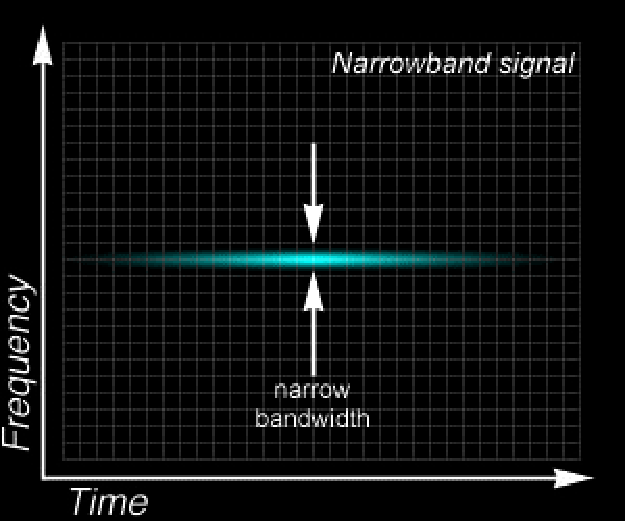
\includegraphics[width=0.35\textwidth]{figures/narrow.pdf}
        \caption{Example of a Gaussian narrowband
        signal~\cite{hid-sp18-601-www-sathome-howworks}}\label{broadbandfigure}
\end{figure*}
 
 If the alien signal is transmitting any kind of information it will probably 
 have it's strength modulated~\cite{hid-sp18-601-book-gray1961radio}, that is
 how AM and PM radio works. SET$@$Home program has to look for this kind of 
 signal as well because of 
 this~\cite{hid-sp18-601-www-sathome-howworks}, increasing the process 
 complexity greatly.

\begin{figure*}[!htb]
        \centering
        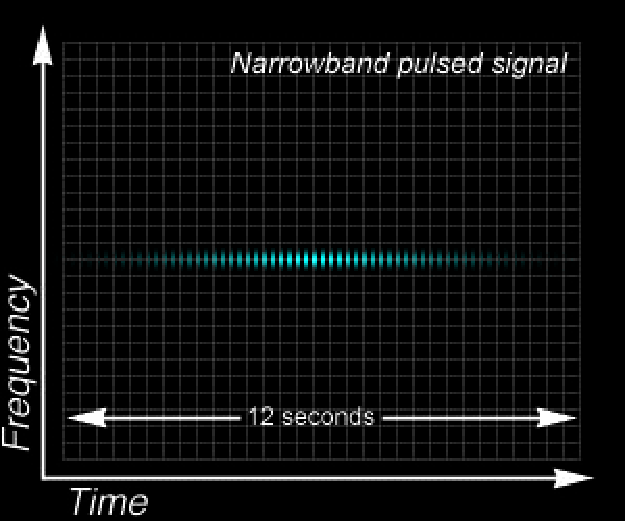
\includegraphics[width=0.35\textwidth]{figures/narrow_pulsed.pdf}
        \caption{Example of a Gaussian pulsed narrowband
        signal~\cite{hid-sp18-601-www-sathome-howworks}}\label{narrowbandfigure}
\end{figure*}

 A kind of distortion that will happen to signals that have traveled to Earth
 is Doppler shift~\cite{hid-sp18-601-www-doppler-light}. Doppler shift is an 
 effect that happens to waves when the 
 source is moving relative to the receiver~\cite{hid-sp18-601-www-doppler}. 
 It shifts the apparent frequency 
 of the wave, meaning that the signal's starting frequency will differ from its 
 ending frequency. SETI$@$home software has to account for this and do what 
 is called ``de-chirping'', reverting the frequency change. However, as the 
 amount of Doppler shift is unknown  the software has to ``de-chirp'' for
 several  different amounts of shift~\cite{hid-sp18-601-www-sathome-howworks}.

\begin{figure*}[!htb]
        \centering
        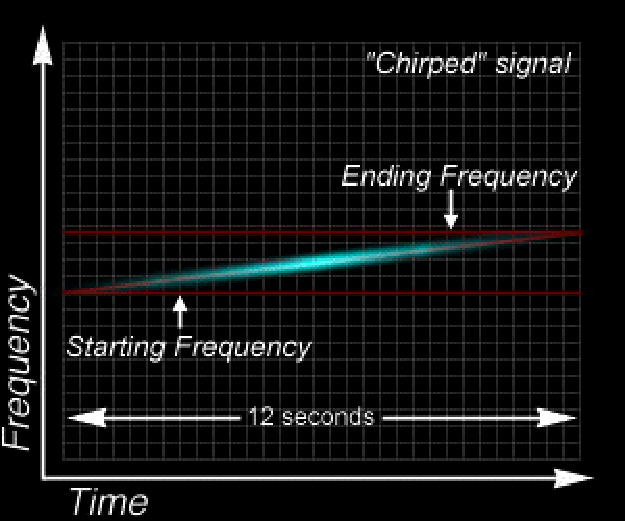
\includegraphics[width=0.35\textwidth]{figures/narrow_chirped.pdf}
        \caption{Example of a Doppler shifted Gaussian narrowband
        signal~\cite{hid-sp18-601-www-sathome-howworks}}\label{dopplerfigure}
\end{figure*}

\subsection{Nodes work}\label{hid-sp18-601-subsection-nodes-work}
The results that the nodes are looking for are candidates for alien signals.
This candidates have to have positives from multiple machines and are then 
verified by the SETI$@$home team in 
Berkeley~\cite{hid-sp18-601-www-sathome-howworks}.

Once the nodes have their data they start the analysis by fixing possible 
Doppler shifts. This is the most time consuming task, as the signal needs to be 
broken down into units of Hz and nHz, this units are $10^{-3}$ to $10^{-6}$ 
times smaller than the original signal, and shifter by a few 
nHz~\cite{hid-sp18-601-www-sathome-howworks}. Once the signal is free of Doppler
 effects the node starts to search for a signal compatible with an 
extra-terrestrial source
~\cite{hid-sp18-601-www-sathome-howworks,hid-sp18-601-paper-cocconi1959searching}.

This very fine Doppler de-shifting may actually over shift the 
signal~\cite{hid-sp18-601-www-sathome-howworks}, so the whole
process is done again with a less fine de-shifting. This is done until the 
de-shifting
is done in units of 1200Hz. This first set of analysis totals over 275 billion 
operations for one work unit.

Signals that show a possibility of being of extra-terrestrial, \textit{i.e.} 
have a strong power for a combination of the aforementioned parameters, are then 
 checked for human contamination. The signal must be 
a Gaussian with a 12 second period~\cite{hid-sp18-601-paper-anderson2002seti} as
mentioned in Subsection~\ref{hid-sp18-601-subsection-signal}.

This process is only for finding continuous signals, as the extra-terrestrial 
signals could be pulsating. This means that special tests have to be applied 
to the signal~\cite{hid-sp18-601-www-sathome-howworks}. One of said tests is 
to look for triplets of peaks, the other test
used was developed by the SET$@$Home team. It's a modification of the 
``fast folding algorithm''~\cite{hid-sp18-601-paper-korpela2001seti}.
This algorithm is capable of detecting signals that would be lost in the noise.

In total, a node will perform between 2.5 trillion and 3.8 trillion operations 
for each work unit~\cite{hid-sp18-601-www-sathome-howworks}. 
This massive amount of operations can only be realistically 
be done by either a super-computer (costly) or a huge cloud of computers. As the
 computers are volunteers this method has almost no cost.

\section{Conclusion}\label{hid-sp18-601-section-conclusions}

SET$@$Home may not have yet found signs of extra terrestrial intelligence, it 
has, however, managed to spurt the volunteer cloud computing movement. Over 50
research initiatives use distributed 
computing~\cite{hid-sp18-601-www-boinc-projects}.

The search for the alien signals might have some more issues with. As was 
mentioned in~\ref{hid-sp18-601-subsection-signal} the kind of signals being 
analyzed have only a single frequency, therefore signals that have frequency 
modulation would not be caught by this method. This includes FM radio and 
digital radio signals. SET$@$Home has been asked about this concerns but has 
yet to comment.




\bibliographystyle{ACM-Reference-Format}
\bibliography{report} 

